\chapter{CONCEPTION ET DÉVELOPPEMENT D\textquotesingle UN JUMEAU NUMÉRIQUE INTÉGRANT L\textquotesingle INTELLIGENCE ARTIFICIELLE}

\section{Introduction}

Après avoir présenté, dans le premier chapitre, les fondements
théoriques relatifs aux réseaux de distribution d\textquotesingle eau
potable, aux technologies de l\textquotesingle Internet des objets
(IoT), aux jumeaux numériques et à l\textquotesingle intelligence
artificielle, puis décrit, dans le deuxième chapitre, la démarche
méthodologique adoptée pour cette recherche, le présent chapitre est
consacré à la conception et au développement de la solution proposée. Il
constitue le cœur technique de cette étude, dans la mesure où il décrit
les différentes étapes ayant conduit à la réalisation
d\textquotesingle un jumeau numérique intégrant
l\textquotesingle intelligence artificielle destiné à améliorer la surveillance et la maintenance, la surveillance et la maintenance du réseau de fourniture
d\textquotesingle eau potable de la commune de Kadutu. Cette phase
traduit les résultats de l\textquotesingle analyse en une solution
informatique concrète répondant aux besoins identifiés auprès des
gestionnaires du réseau du réseau d\textquotesingle eau potable \cite{ref106}.

La conception d\textquotesingle un système informatique de cette nature
nécessite une approche structurée permettant d\textquotesingle assurer
la cohérence entre les besoins des utilisateurs, les choix
technologiques et les fonctionnalités développées. Dans cette étude, le
système est conçu selon une architecture modulaire facilitant
l\textquotesingle intégration de plusieurs technologies complémentaires,
notamment React.js (Vite avec JSX) pour l\textquotesingle interface
utilisateur, FastAPI pour les services backend, SQLite pour la gestion
des données et des algorithmes d\textquotesingle intelligence
artificielle développés en Python pour l\textquotesingle analyse
prédictive et la détection des anomalies. Cette architecture garantit
une meilleure évolutivité du système tout en facilitant son déploiement
et sa maintenance \cite{ref114}.

Le jumeau numérique développé vise à reproduire virtuellement le
fonctionnement du réseau physique de distribution d\textquotesingle eau
potable grâce à l\textquotesingle exploitation des données collectées
par des capteurs intelligents. Ces données, relatives notamment à la
pression, au débit, au niveau d\textquotesingle eau, à la qualité de
l\textquotesingle eau et à l\textquotesingle état des équipements, sont
analysées en temps réel afin d\textquotesingle identifier les anomalies,
de prévoir certaines défaillances et de fournir aux gestionnaires du réseau des
informations facilitant la prise de décision.
L\textquotesingle intégration de l\textquotesingle intelligence
artificielle permet d\textquotesingle améliorer les capacités
d\textquotesingle analyse du système en exploitant les données
historiques et les données instantanées pour générer des prédictions
fiables concernant le comportement du réseau \cite{ref17}.

Dans ce chapitre, seront successivement présentés
l\textquotesingle analyse détaillée du système proposé, la conception de
l\textquotesingle architecture générale, la modélisation UML, la
conception de la base de données, le développement des différents
modules logiciels, l\textquotesingle intégration de
l\textquotesingle intelligence artificielle, la réalisation des
interfaces utilisateur ainsi que les tests effectués pour valider le
fonctionnement du prototype. L\textquotesingle objectif est de démontrer
que la solution développée répond aux exigences fonctionnelles et
techniques identifiées tout au long de cette recherche et
qu\textquotesingle elle constitue une contribution pertinente à la
modernisation de la gestion des réseaux de distribution
d\textquotesingle eau potable \cite{ref106}, \cite{ref17}.

\section{Analyse détaillée du système proposé}\label{analyse-duxe9tailluxe9e-du-systuxe8me-proposuxe9}

L\textquotesingle analyse détaillée du système proposé consiste à
définir de manière précise les caractéristiques fonctionnelles et
techniques du jumeau numérique développé dans le cadre de cette étude.
Cette étape permet de traduire les besoins identifiés lors de
l\textquotesingle analyse du système existant en une solution
informatique cohérente répondant aux exigences des gestionnaires du réseau du
réseau de fourniture d\textquotesingle eau potable de la commune de
Kadutu. Elle constitue un pont entre les résultats de
l\textquotesingle analyse des besoins présentés au chapitre précédent et
les activités de conception et de développement du système. Une analyse
détaillée facilite la conception d\textquotesingle une architecture
logicielle adaptée et réduit les risques d\textquotesingle incohérence
lors de l\textquotesingle implémentation de la solution \cite{ref106}.

Le système proposé est conçu comme une plateforme intelligente reposant
sur le concept du \textbf{jumeau numérique}. Il s\textquotesingle agit
d\textquotesingle une représentation virtuelle dynamique du réseau de
fourniture d\textquotesingle eau potable, alimentée en continu par les
données issues des capteurs installés sur les différentes
infrastructures hydrauliques. Cette représentation numérique reproduit
le comportement du réseau physique en temps réel et permet aux
gestionnaires du réseau de suivre l\textquotesingle état des équipements,
d\textquotesingle observer les paramètres hydrauliques, de détecter les
anomalies et de simuler différents scénarios de fonctionnement.
L\textquotesingle intégration de l\textquotesingle intelligence
artificielle permet en outre d\textquotesingle exploiter les données
collectées afin de produire des analyses prédictives et
d\textquotesingle améliorer la prise de décision \cite{ref17}.

Le développement du système répond principalement aux insuffisances
constatées dans les méthodes traditionnelles de gestion du réseau de
distribution d\textquotesingle eau potable, caractérisées par une
surveillance essentiellement manuelle, une maintenance souvent
corrective et une faible capacité d\textquotesingle anticipation des
défaillances. En proposant une plateforme centralisée intégrant la
visualisation en temps réel, l\textquotesingle analyse intelligente des
données et la gestion des alertes, le système contribue à améliorer la
disponibilité des informations, la rapidité des interventions techniques
et l\textquotesingle efficacité globale de
l\textquotesingle exploitation du réseau \cite{ref20}.

\subsection{Objectif du système proposé}\label{objectif-du-systuxe8me-proposuxe9}

Le système développé a pour objectif de fournir aux gestionnaires du réseau de la
REGIDESO un outil numérique capable d\textquotesingle assurer la
surveillance en temps réel du réseau de fourniture d\textquotesingle eau
potable de la commune de Kadutu, de détecter automatiquement les
anomalies, de prédire certaines défaillances grâce à
l\textquotesingle intelligence artificielle et
d\textquotesingle assister les équipes techniques dans les opérations de
maintenance et de planification du réseau. Il vise également à améliorer
la qualité du service offert aux abonnés en réduisant les pertes
d\textquotesingle eau et les interruptions de distribution \cite{ref17}.

\subsection{Description générale du système}\label{description-guxe9nuxe9rale-du-systuxe8me}

Le jumeau numérique proposé est constitué de plusieurs modules
interconnectés qui collaborent afin d\textquotesingle assurer le
fonctionnement global de la plateforme.

Le premier module correspond à la \textbf{collecte des données}, assurée
par des capteurs intelligents mesurant différents paramètres du réseau
tels que la pression, le débit, le niveau des réservoirs, la qualité de
l\textquotesingle eau et l\textquotesingle état des équipements.

Le deuxième module est le \textbf{serveur applicatif}, développé avec
\textbf{FastAPI}, qui reçoit les données des capteurs, les traite, les
enregistre dans la base de données et les met à disposition des autres
composants du système.

Le troisième module est constitué du \textbf{moteur
	d\textquotesingle intelligence artificielle}, chargé
d\textquotesingle analyser les données historiques et instantanées afin
de détecter les anomalies, d\textquotesingle estimer les risques de
panne et de identifier les situations anormales et fournir des informations utiles
à la maintenance.

Le quatrième module correspond à \textbf{l\textquotesingle interface
	utilisateur}, développée avec \textbf{React.js (Vite - JSX)}, qui permet
aux utilisateurs de consulter le jumeau numérique, les cartes
interactives, les tableaux de bord, les alertes, les statistiques ainsi
que les rapports générés par le système.

L\textquotesingle ensemble de ces modules communique au moyen
d\textquotesingle API REST, garantissant une architecture modulaire,
évolutive et facilement maintenable \cite{ref114}.

\subsection{Principales fonctionnalités}\label{principales-fonctionnalituxe9s}

Le système développé offre notamment les fonctionnalités suivantes :

\begin{itemize}
	\item
	authentification sécurisée des utilisateurs ;
	\item
	visualisation du réseau sur une carte interactive ;
	\item
	représentation numérique dynamique du réseau de distribution
	d\textquotesingle eau ;
	\item
	affichage des données du réseau et actualisation des informations via
	les API REST ;
	\item
	surveillance de la pression, du débit, du niveau et de la qualité de
	l\textquotesingle eau ;
	\item
	détection automatique des fuites et des anomalies ;
	\item
	prédiction des pannes grâce aux algorithmes
	d\textquotesingle intelligence artificielle ;
	\item
	génération d\textquotesingle alertes et de notifications ;
	\item
	suivi des interventions de maintenance ;
	\item
	consultation des statistiques et indicateurs de performance ;
	\item
	gestion des utilisateurs et des équipements ;
	\item
	génération de rapports d\textquotesingle exploitation.
\end{itemize}

Ces fonctionnalités répondent directement aux besoins exprimés par les
gestionnaires du réseau du réseau et contribuent à une gestion plus efficace des
infrastructures hydrauliques \cite{ref106}\textbf{,} \cite{ref20}.

\subsection{Valeur ajoutée du système}\label{valeur-ajoutuxe9e-du-systuxe8me}

Contrairement aux systèmes traditionnels de supervision, la solution
proposée intègre simultanément les technologies des jumeaux numériques,
de l\textquotesingle Internet des objets et de
l\textquotesingle intelligence artificielle dans une plateforme unique.
Cette intégration permet non seulement d\textquotesingle observer le
fonctionnement du réseau en temps réel, mais également
d\textquotesingle anticiper les défaillances, de simuler différents
scénarios de fonctionnement et d\textquotesingle assister les décideurs
dans la planification des opérations de maintenance. Le système
constitue ainsi un outil d\textquotesingle aide à la décision
susceptible d\textquotesingle améliorer la performance globale du réseau
de distribution d\textquotesingle eau potable de la commune de Kadutu
\cite{ref17}\textbf{,} \cite{ref114}.

\section{Conception du système}

La conception du système constitue une étape fondamentale dans le
développement d\textquotesingle une application informatique, car elle
permet de définir l\textquotesingle organisation des différents
composants logiciels et matériels avant leur implémentation. Elle assure
une meilleure compréhension du fonctionnement global de la solution
proposée et facilite son développement, sa maintenance ainsi que son
évolution future. Dans cette étude, la conception est réalisée selon une
architecture modulaire intégrant les technologies du jumeau numérique,
de l\textquotesingle Internet des objets (IoT) et de
l\textquotesingle intelligence artificielle afin de répondre
efficacement aux besoins de surveillance, de maintenance et
d\textquotesingle optimisation du réseau de fourniture
d\textquotesingle eau potable de la commune de Kadutu \cite{ref106}.

L\textquotesingle architecture proposée est organisée autour de
plusieurs couches indépendantes mais interconnectées, permettant une
circulation fluide des données depuis les capteurs installés sur le
réseau physique jusqu\textquotesingle à l\textquotesingle interface de
visualisation utilisée par les gestionnaires du réseau. Cette organisation
favorise la séparation des responsabilités entre les différents modules,
améliore les performances du système et facilite
l\textquotesingle intégration de nouvelles fonctionnalités sans modifier
l\textquotesingle ensemble de l\textquotesingle application \cite{ref114}.

\subsection{Architecture générale du système}

L\textquotesingle architecture générale du système repose sur cinq
grandes composantes fonctionnelles qui collaborent afin
d\textquotesingle assurer le fonctionnement du jumeau numérique.

Les principales composantes sont :

\begin{itemize}
	\item
	le réseau physique de distribution d\textquotesingle eau potable ;
	\item
	les sources de données et capteurs (réels ou simulés) ;
	\item
	le serveur applicatif ;
	\item
	le moteur d\textquotesingle intelligence artificielle ;
	\item
	l\textquotesingle application Web représentant le jumeau numérique.
\end{itemize}

Les informations circulent de manière continue entre ces différents
composants afin de permettre une représentation fidèle de
l\textquotesingle état du réseau en temps réel. Les données collectées
par les capteurs sont analysées puis affichées sous forme de tableaux de
bord, de cartes interactives et d\textquotesingle indicateurs de
performance destinés aux gestionnaires du réseau \cite{ref17}.

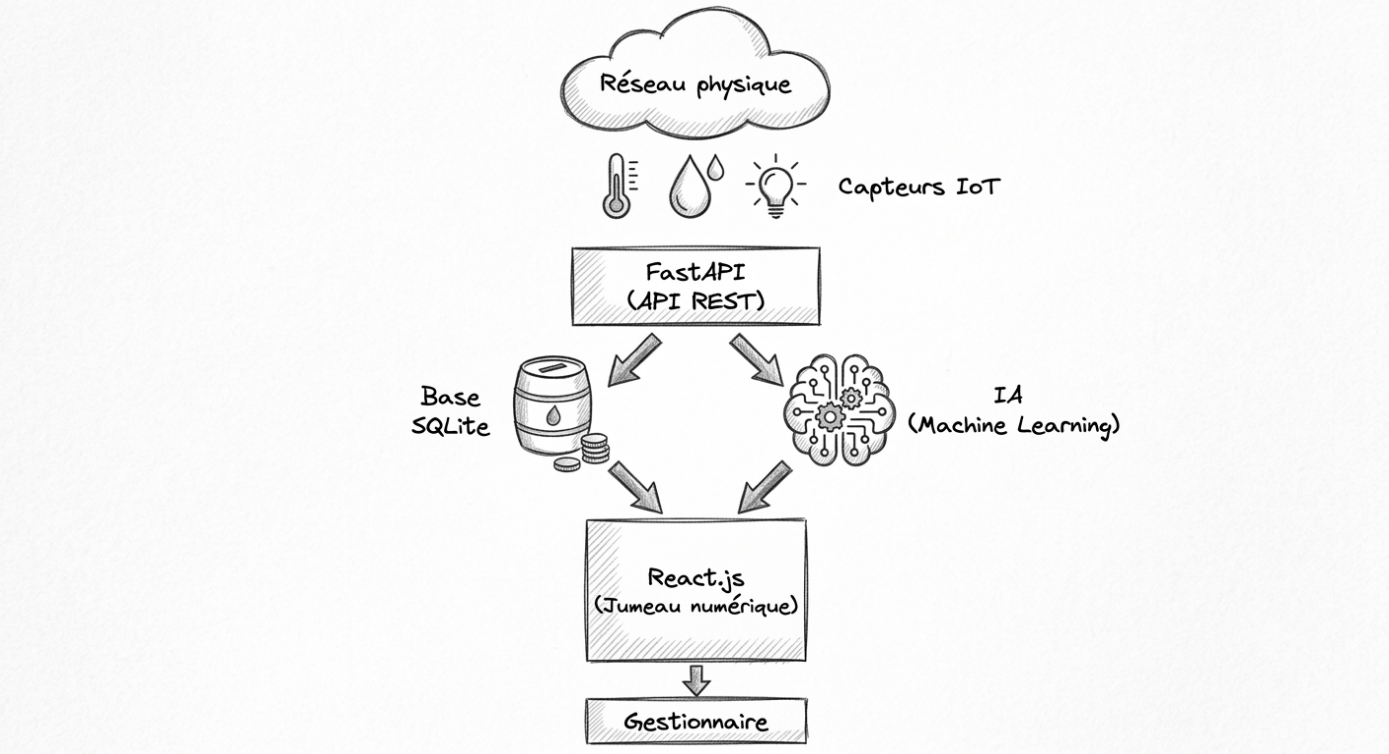
\includegraphics[width=6.3in,height=3.43571in]{figures/image3.png}

Figure 3 Architecture générale du système proposé

\subsection{Architecture physique}

L\textquotesingle architecture physique représente les équipements
matériels intervenant dans le fonctionnement du système.

Elle comprend principalement :

\begin{itemize}
	\item
	les infrastructures hydrauliques (réservoirs, conduites, stations de
	pompage) ;
	\item
	les capteurs intelligents installés sur le réseau ;
	\item
	le serveur hébergeant l\textquotesingle API et la base de données ;
	\item
	les ordinateurs utilisés par les gestionnaires du réseau ;
	\item
	la connexion réseau permettant la communication entre les différents
	composants.
\end{itemize}

Cette architecture permet d'intégrer les données disponibles au
prototype et de les transmettre vers la plateforme numérique pour leur
exploitation \cite{ref20}.

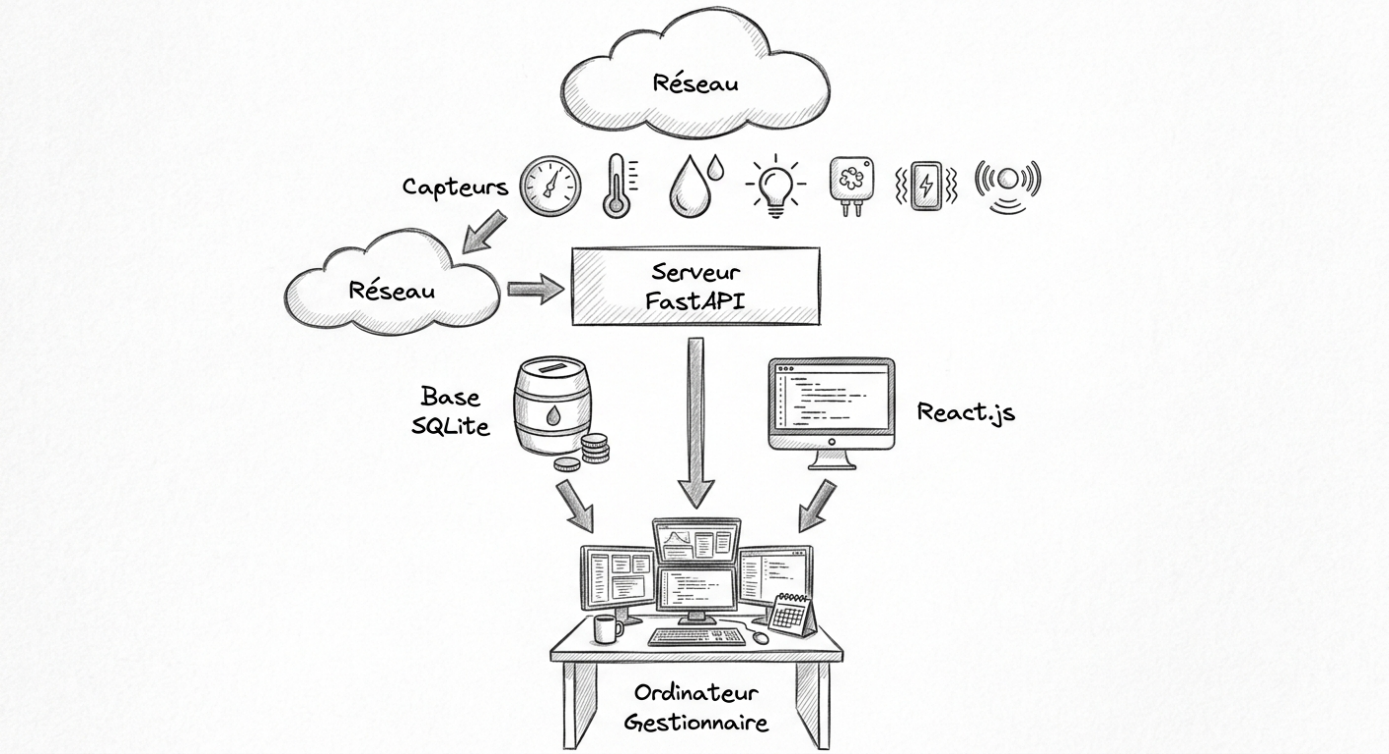
\includegraphics[width=6.3in,height=3.43571in]{figures/image4.png}

Figure 4 Architecture physique

\subsection{Architecture logicielle}\label{architecture-logicielle}

L\textquotesingle application est développée selon une architecture en
couches (\emph{Layered Architecture}), permettant de séparer clairement
les différentes responsabilités.

Elle est composée de :

\subsubsection{Couche de présentation}\label{couche-de-pruxe9sentation}

Développée avec \textbf{React.js (Vite - JSX)}, cette couche permet aux
utilisateurs de visualiser les informations du réseau, les cartes
interactives, les statistiques et les alertes.

\subsubsection{Couche métier}\label{couche-muxe9tier}

Cette couche est développée avec \textbf{FastAPI}. Elle contient toute
la logique métier, notamment :

\begin{itemize}
	\item
	gestion des utilisateurs ;
	\item
	gestion des équipements ;
	\item
	traitement des données ;
	\item
	communication avec l\textquotesingle IA ;
	\item
	génération des alertes.
\end{itemize}

\subsubsection{Couche intelligence
	artificielle}\label{couche-intelligence-artificielle}

Elle réalise :

\begin{itemize}
	\item
	la détection des anomalies ;
	\item
	la prédiction des pannes ;
	\item
	l\textquotesingle analyse des tendances ;
	\item
	les recommandations de maintenance.
\end{itemize}

\subsubsection{Couche données}\label{couche-donnuxe9es}

Cette couche correspond à \textbf{SQLite}, qui stocke :

\begin{itemize}
	\item
	utilisateurs ;
	\item
	capteurs ;
	\item
	équipements ;
	\item
	mesures ;
	\item
	alertes ;
	\item
	historiques.
\end{itemize}

L\textquotesingle utilisation d\textquotesingle une architecture
multicouche améliore la modularité, facilite la maintenance et permet de
faire évoluer indépendamment chaque composant du système \cite{ref106}.

\subsection{Architecture fonctionnelle}\label{architecture-fonctionnelle}

L\textquotesingle architecture fonctionnelle décrit les principaux
traitements réalisés par le système.

Le fonctionnement général est le suivant :

\begin{enumerate}
	\def\labelenumi{\arabic{enumi}.}
	\item
	Les sources de données fournissent les mesures ou valeurs simulées des
	paramètres du réseau.
	\item
	Les données sont transmises au serveur FastAPI à travers les API REST.
	\item
	Les informations sont enregistrées dans la base de données.
	\item
	Le moteur d\textquotesingle intelligence artificielle analyse les
	mesures.
	\item
	Les anomalies sont détectées.
	\item
	Les alertes sont générées.
	\item
	Les résultats sont affichés sur le jumeau numérique.
	\item
	Les gestionnaires du réseau prennent les décisions nécessaires.
\end{enumerate}

Cette organisation facilite la surveillance du réseau et l'analyse des
anomalies \cite{ref17}.

\subsection{Architecture de déploiement}\label{architecture-de-duxe9ploiement}

Le système est conçu selon une architecture client-serveur.

Le serveur héberge :

\begin{itemize}
	\item
	FastAPI ;
	\item
	SQLite ;
	\item
	le modèle d\textquotesingle intelligence artificielle ;
	\item
	les API REST.
\end{itemize}

Les clients utilisent simplement un navigateur Web.

L\textquotesingle interface React.js communique avec FastAPI via
\textbf{Axios}, qui envoie des requêtes HTTP pour récupérer ou
transmettre les données.

Cette architecture permet un déploiement aussi bien sur un serveur local
que sur un serveur cloud sans modification majeure de
l\textquotesingle application \cite{ref114}.

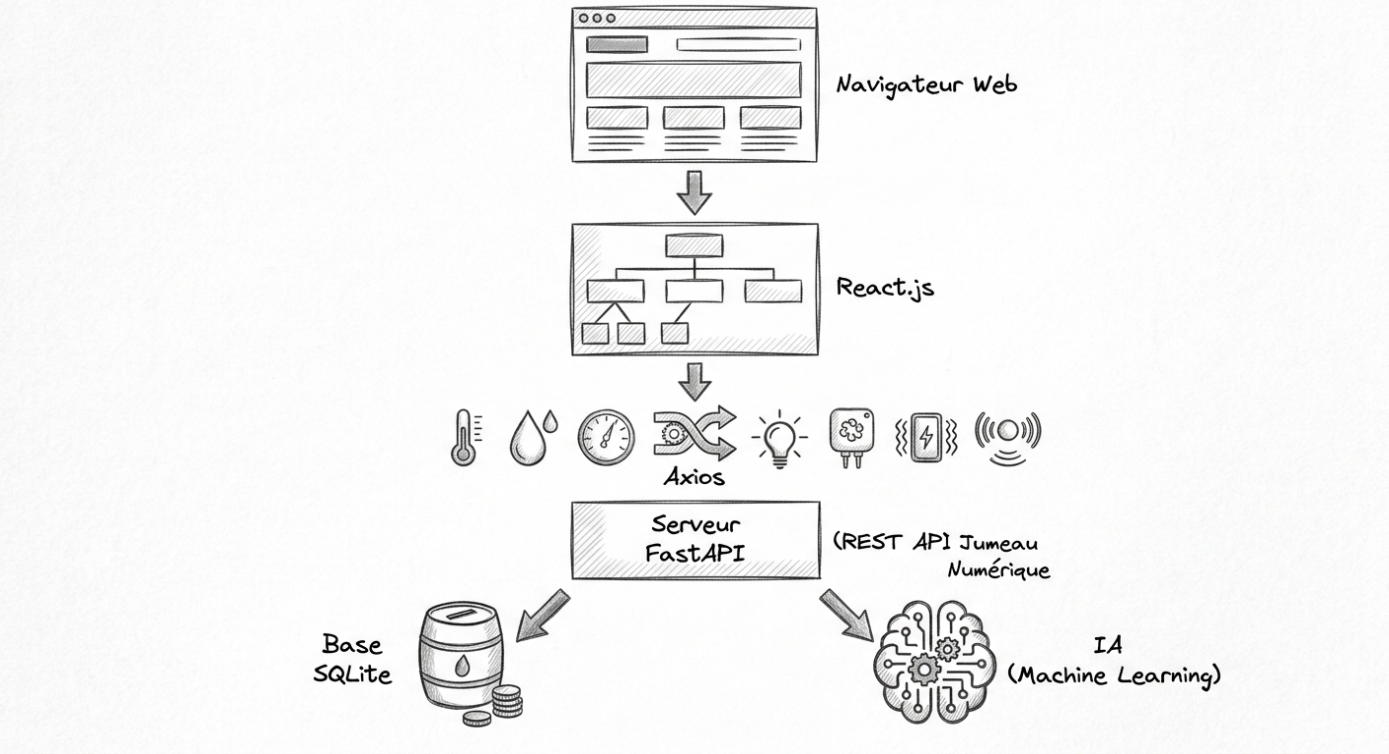
\includegraphics[width=6.3in,height=3.43571in]{figures/image5.png}

Figure 5 Architecture de déploiement

\clearpage